
\section{Heurística e Ciclo}

%->8-------------------------------------------------------------------------------------------8<-%
\begin{frame}[fragile]
  \frametitle{Heurística}
  \begin{itemize}
    \item Sabemos resolver $\argmin{Q,t} \fnorm{Q\blue{A} .+ t e\t - \red{B}}$; \vspace{1cm}
    \item Sabemos resolver $\argmin{P} \fnorm{\blue{A} - \red{B}P}$; \vspace{1cm}
    \item Mas não sabemos resolver $\argmin{Q,t,P} \fnorm{Q\blue{A} .+ t e\t - \red{B}P}.$
  \end{itemize}
  \vspace{1cm}
  \begin{center}
    Heurística!
  \end{center}
\end{frame}
%->8-------------------------------------------------------------------------------------------8<-%

\begin{frame}
  \frametitle{Cíclo}
  \begin{figure}
    \centering
    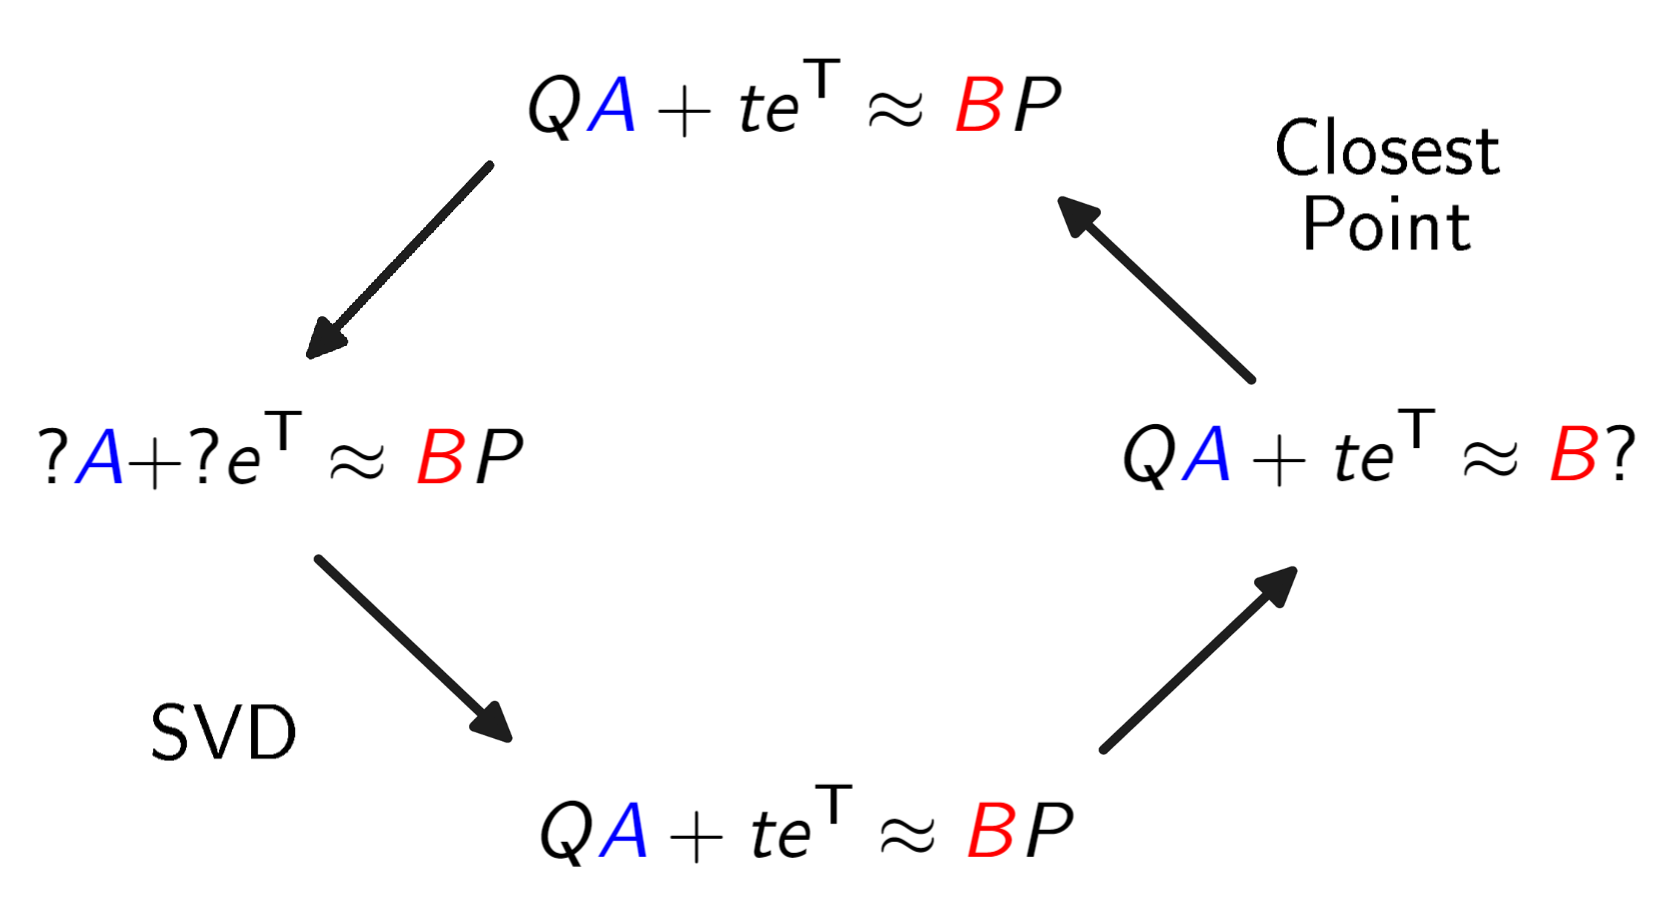
\includegraphics[width=1\textwidth]{cycle.png}
  \end{figure}
\end{frame}

\begin{frame}[fragile]
  \frametitle{Código}
  \begin{code}
    function point_matching(A, B; iters = 100)
      P = zeros(size(B, 2), size(A, 2))
      Q = I(size(A, 1))
      t = zeros(size(A, 1))

      for _ in 1:iters
        P = best_indicator(Q*A .+ t, B)
        Q, t = best_rigid_transf(A, B*P)
      end

      return P, Q, t
    end
  \end{code}
\end{frame}
